% Este arquivo .tex será incluído no arquivo .tex principal. Não é preciso
% declarar nenhum cabeçalho

\section{Iniciação Científica}

A Iniciação Científica é um tempo para o aluno de graduação (você, no caso) ter
uma experiência acadêmica mais séria, sentir um pouco como é o clima de
pesquisa. Interessou? O que fazer? Calma, você mal entrou na Universidade.
Geralmente, o que se faz é conversar com o professor da área com a qual você se
identifica mais (criptografia, teoria da computação, processamento de imagens,
inteligência artificial etc.) e ver se ele está desenvolvendo algum projeto
interessante naquela área, ou propor para ele alguma ideia sua mesmo.  Depois
você começa a estudar para redigir um projeto e encaminhá-lo para alguma
instituição de fomento à pesquisa (CNPq ou FAPESP), pedindo uma bolsa de
Iniciação Científica. A FAPESP paga em torno de R\$520,00 e aceita pedidos de
bolsa em qualquer período do ano. O CNPq paga aproximadamente R\$400,00, e o
período para inscrição de projetos é geralmente em junho e novembro. No primeiro
semestre geralmente é bem mais difícil achar algum professor da área que você se
interessa, aliás, é bem difícil saber a área com a qual você se identifica, pois
você mal começou o curso e não conhece muito do que se estuda em Computação,
muito menos os professores. Mas tenha paciência, agora parece tudo muito
complicado, mas com o tempo as coisas vão ficando mais simples. Se você
realmente tiver uma sede insaciável de conhecer o meio da pesquisa, procure o
seu professor de MC102, ele pode te orientar a respeito.

\begin{figure}[h!]
    \centering
    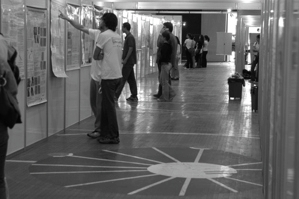
\includegraphics[width=.45\textwidth]{img/unicamp/congresso.jpg}
    \caption{Congresso de Iniciação Científica da Unicamp}
\end{figure}

Outra coisa interessante a respeito da Iniciação Científica é que, se você
conseguir bolsa (o que não é muito difícil), pode pegar a disciplina MC040 e
posteriormente MC041 (2 semestres), cada uma com 12 créditos, e geralmente se
tira notas altas nessas disciplinas. Ou seja, são 24 créditos praticamente ``de
bandeja'' para aumentar o seu CR, ou ajudar a recuperá-lo, caso esteja no fundo
do poço. Note bem as aspas. Os trabalhos de Iniciação Científica geralmente
consomem muito tempo de estudo e dedicação, não vá pensando que é moleza não.

Na FEEC você pode conseguir as matérias de Iniciação (EA002 até EA005) mesmo sem
bolsa, mas você ainda assim vai precisar de um orientador. Lá a Iniciação
Científica também substitui o estágio, mas não tem equivalência com as do IC.
